%\documentclass{beamer}
\documentclass[handout]{beamer}
\usetheme{boxes} 
%\usetheme{default}

%math fonts
%\renewcommand\mathfamilydefault{\rmdefault}

%page numbers
\setbeamertemplate{footline}[page number]
\setbeamertemplate{section in head/foot}{\hfill\insertsectionheadnumber.~\insertsectionhead}
\setbeamertemplate{section in head/foot shaded}{\color{structure!50}\hfill\insertsectionheadnumber.~\insertsectionhead}
\setbeamertemplate{section in toc}{\inserttocsectionnumber.~\inserttocsection}

\setbeamercovered{invisible}
\setbeamertemplate{navigation symbols}{} 
\usepackage{mathtools}
\usepackage{graphicx}
\usepackage{amsmath}
\usepackage{epstopdf}
\usepackage{color}

%embed videos
\usepackage{media9}

\title[Robust Control]{Bootstrap Yourself to $H_{\infty}$ in 15 Minutes}
\author{Okan Ko\c{c}}
\institute[IAS]
{
MPI for Intelligent Systems, T\"ubingen \\
Robot Learning Lab \\
\medskip
{\emph{okan.koc@tuebingen.mpg.de}}
}
\date{\today}

% Set the paths where all figures are taken from:
\graphicspath{{Pictures/}}
\mathtoolsset{showonlyrefs} 
\newcommand{\includesvg}[1]{%
% \executeiffilenewer{#1.svg}{#1.pdf}%
% {inkscape -z -D --file=#1.svg %
% --export-pdf=#1.pdf --export-latex}%
 \input{#1.pdf_tex}%
}

\begin{document}
%
\begin{frame}
\titlepage
\end{frame}
%
\begin{frame}
\frametitle{Table of Contents}
\tableofcontents
\end{frame}
%
\section{Motivation: Table Tennis}
%
\begin{frame}{300 Years of Optimal Control}
\begin{columns}
\begin{column}{.49\textwidth}
\begin{itemize}
\item I worry that I cannot condense 300 years of Optimal Control to 15 Minutes!
\item Alternative Title:
\item How I Learned to Stop Worrying and Love Table Tennis!
\end{itemize}
\end{column}
\begin{column}{.49\textwidth}
\begin{figure}
\center
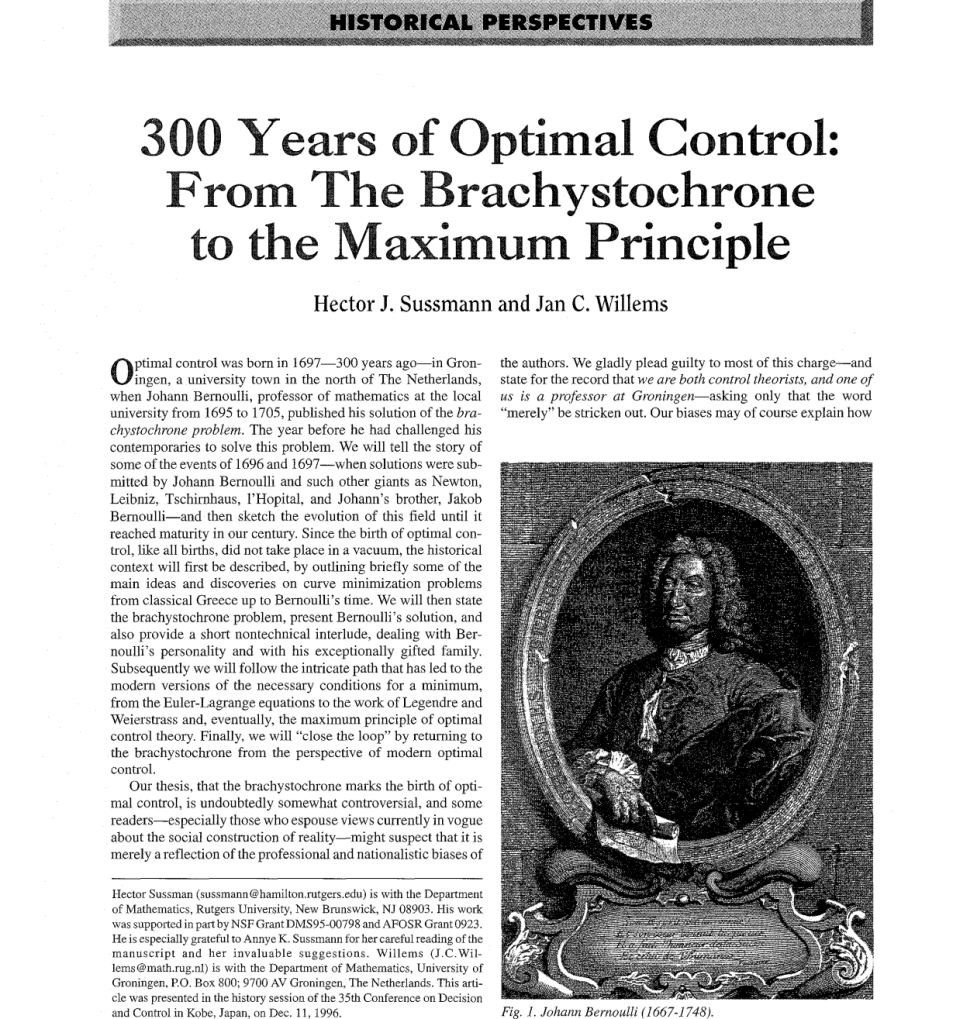
\includegraphics[scale=0.3, angle= 0]{300YearsOfOptimalControl.png}			
\caption{A Historical Perspective on Optimal Control~\cite{Sussmann97}}
\end{figure}
\end{column}
\end{columns}
\end{frame}
%
\begin{frame}{Overview}
\begin{itemize}
\item Robustness in Table Tennis
\item Linear Quadratic Regulator (LQR/LQG)
\item Generalized Plant
\item Mention of $H_{\infty}$ techniques
\item How to apply to table tennis?
\end{itemize}
\end{frame}
%
\begin{frame}{Example from Professional Table Tennis}
\includemedia[
width=0.6\linewidth,height=0.3375\linewidth, % 16:9
activate=pageopen,
flashvars={
modestbranding=1 % no YT logo in control bar
&autohide=1 % controlbar autohide
&showinfo=0 % no title and other info before start
&rel=0 % no related videos after end
}
]{}{https://www.youtube.com/watch?v=8x45dAA3wxM}
\end{frame}
%
\begin{frame}{Table Tennis}
\begin{itemize}
\item Difficult to predict in advance speed and direction of incoming ball
\item High spins make it impossible!
\item Adversary reacts to your strategy!
\item Initial gesture and hitting trajectories should be planned robustly!
\end{itemize}
\end{frame}
%
\begin{frame}{Spin Types}
\begin{figure}
\center
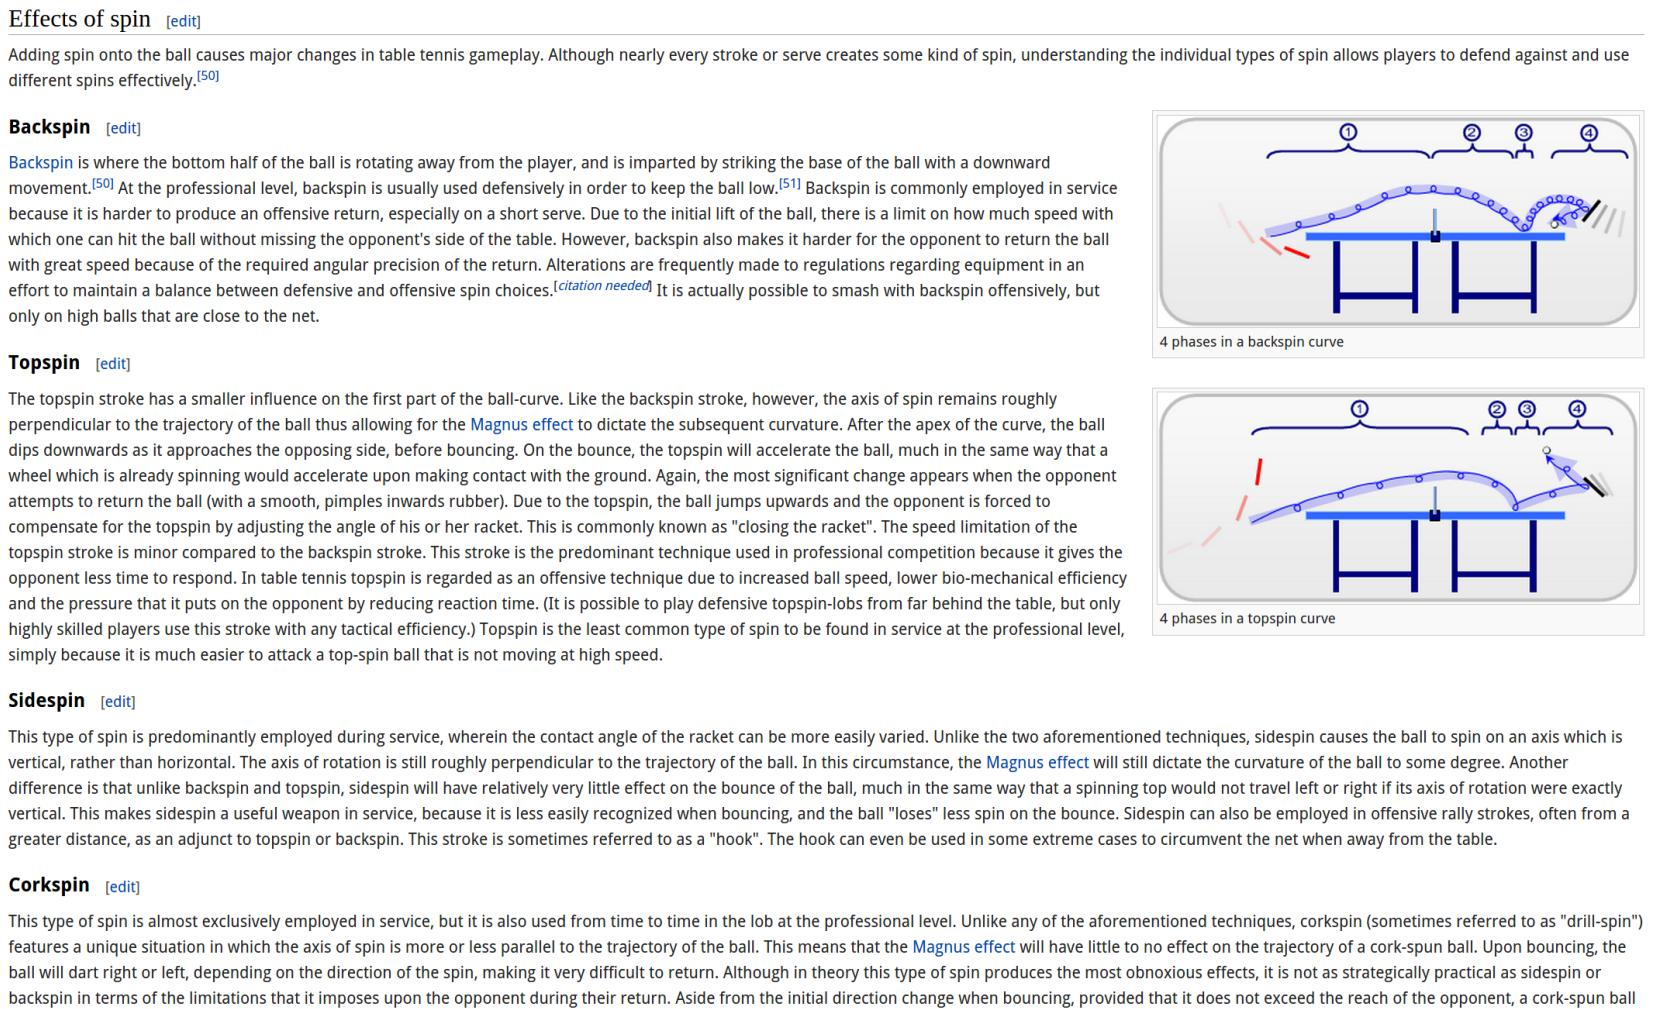
\includegraphics[scale=0.4]{spinTypes.jpg}		
\caption{Different types of spin~\cite{wiki}}
\end{figure}
\end{frame}
%
\begin{frame}{Differential Game}
\begin{columns}
\begin{column}{.49\textwidth}
\begin{itemize}
\item Game theoretic setting due to two player interaction
\end{itemize}
\begin{equation}
\dot{x} = A x + B_1 u + B_2 v
\end{equation}
\begin{itemize}
\item Min-max control policy:
\end{itemize}
\scalebox{0.8}{\parbox{.5\linewidth}{
\begin{equation}
\begin{aligned}
u^{*} &= \arg\min_{u}\max_{v} J(u,v) \\
J(u,v) &= \int e^{\mathrm{T}}Qe + u^{\mathrm{T}}R_u u + v^{\mathrm{T}}R_v v \ \mathrm{d}t \\ 
e(t) &= x(t) - r(t)
\end{aligned}
\end{equation}}} 
\end{column}
\begin{column}{.49\textwidth}
\begin{figure}
\center
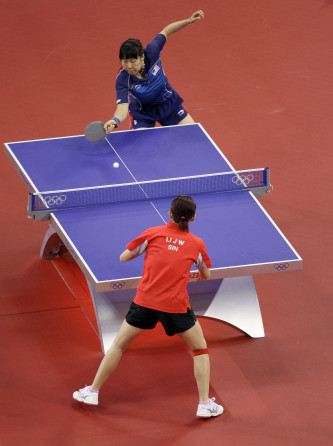
\includegraphics[scale=2.0]{table-tennis.jpg}
\caption{Unexpected things can happen!}
\end{figure}
\end{column}
\end{columns}
\end{frame}
%
\section{Linear Optimal Control}
%
\begin{frame}{Linear Quadratic Regulator (LQR)}
\begin{itemize}
\item Start with the Bellman's equation
\begin{equation*}
\begin{aligned}
J(x) = \min_u c(x,u) + \sum_{x'} \pi_x(x',u)J(x')
\end{aligned}
\end{equation*}
\item Take the limit to obtain the Hamilton-Jacobi-Bellman PDE 
\begin{eqnarray}
\min_u \{ q(x,u) + \frac{\partial J}{\partial x}^{\mathrm{T}}f(x,u) \} + \frac{\partial J}{\partial t} = 0 \\
\dot{x} = f(x,u)
\end{eqnarray}
\item Difficult to solve for nonlinear models or nonquadratic cost functions!
\end{itemize}
\end{frame}
%
\begin{frame}{Linear Quadratic Regulator (LQR)}
\begin{itemize}
\item Analytical solution for linear models with quadratic cost
\end{itemize}
\begin{equation}
\begin{aligned}
\dot{x} &= Ax + Bu \\
J(u) &= \int_{0}^{T} x^{\mathrm{T}}Qx + u^{\mathrm{T}}Ru \ \mathrm{d}t + x(T)Q_{T}x(T) \\
\end{aligned}
\end{equation}
\begin{itemize}
\item as a linear feedback law
\end{itemize}
\begin{equation}
\begin{aligned}
\\
u &= -R^{-1}B^{\mathrm{T}}P(t)x(t) \\
-\dot{P} &= PA + A^{\mathrm{T}}P - PBR^{-1}B^{\mathrm{T}}P + Q \\ 
P(T) &= Q_{T}
\end{aligned}
\end{equation}
\end{frame}
%
\begin{frame}{Robustness to Disturbance}
\begin{itemize}
\item If the system is controllable and detectable LQR feedback ensures closed-loop stability.
\item It also ensures robustness to disturbances
\item Gain and phase margins in Bode or Nyquist plots.
\item Sensitivity $S(jw)$ and complementary sensitivity $T(jw)$.
\end{itemize}
\begin{figure}
\center
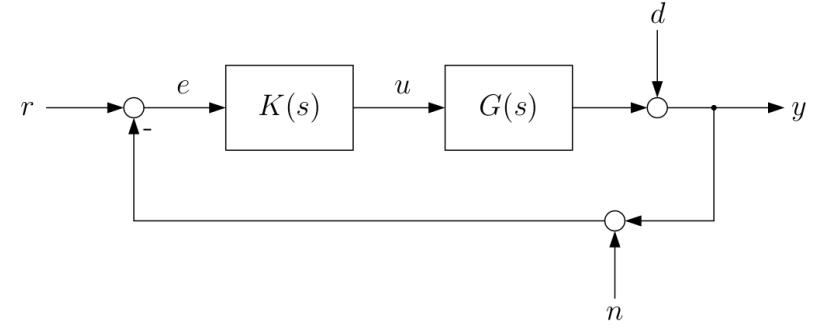
\includegraphics[scale=0.4]{closedLoop.jpg}	
\caption{Closing the loop with feedback}
\end{figure}
\end{frame}
%
\begin{frame}{Robustness to Disturbance}
\begin{itemize}
\item Sensitivity: $S(jw) = (I + GK)^{-1}$
\item Complementary sensitivity: $T(jw) = GK(I + GK)^{-1}$.
\item $y = T(jw)(r - n) + S(jw)d$
\item Good disturbance rejection \& tracking: $\Rightarrow \bar{\sigma}[S(jw)] \ll 1$
\item Good noise rejection \& low sensitivity to unstructured multiplicative plant uncertainty $\Rightarrow \bar{\sigma}[T(jw)] \ll 1$
\end{itemize}
\begin{figure}
\center
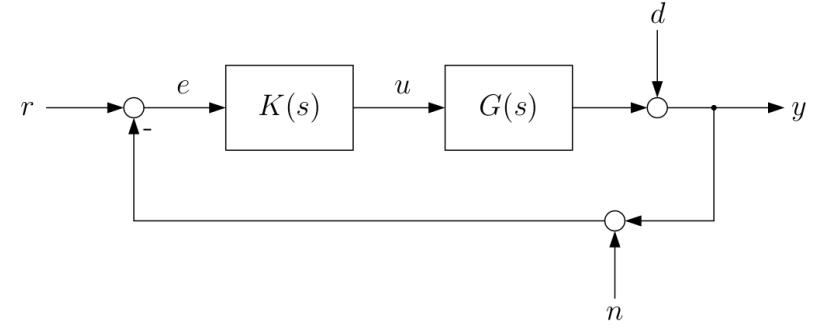
\includegraphics[scale=0.4]{closedLoop.jpg}	
\caption{Closing the loop with feedback}
\end{figure}
\end{frame}
%
\begin{frame}{Optimal State Estimate Feedback (LQG)}
\begin{itemize}
\item Typically one has access to only state estimates!
\end{itemize}
\begin{equation}
\begin{aligned}
\dot{x} &= Ax + Bu + \omega \\
y &= Cx + \nu \\
\end{aligned}
\end{equation}
\begin{itemize}
\item Minimize $J(u) = \mathbb{E}\Big\{\int_{0}^{T} x^{\mathrm{T}}Qx + u^{\mathrm{T}}Ru \ \mathrm{d}t + x(T)Q_{T}x(T)\Big\}$
\item Seperation Principle: $u = -R^{-1}B^{\mathrm{T}}P(t)\hat{x}(t)$
\end{itemize}
\begin{itemize}
\item LQG: Kalman filter in the LQR feedback loop
\end{itemize}
\end{frame}
%
\begin{frame}{Best Abstract Ever}
\begin{columns}
\begin{column}{.49\textwidth}
  \begin{itemize}
   \item What about robustness of LQG?
   \item John Doyle in his famous paper~\cite{Doyle78} shows that LQG can be very sensitive to disturbances by giving a counterexample.
  \end{itemize}
\end{column}
\begin{column}{.49\textwidth}
  \begin{figure}
  \center
  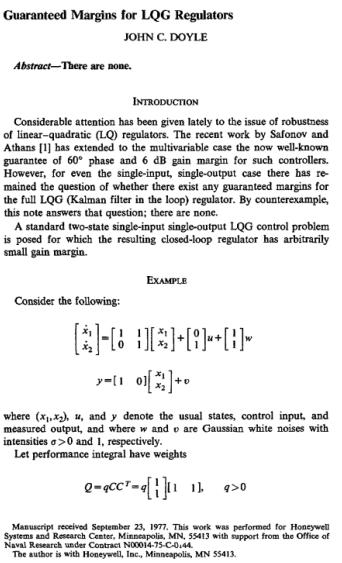
\includegraphics[scale=0.6]{guaranteedMarginsForLQG.jpg}			
  \caption{Guaranteed Margins for LQG: There are none!}
  \end{figure}
\end{column}
\end{columns}
\end{frame}
%
\section{Introducing Robust Control}
%
\begin{frame}{Generalized Plant}
\begin{itemize}
\item Consider the generalized plant dynamics:
\end{itemize}
\begin{figure}
  \center
  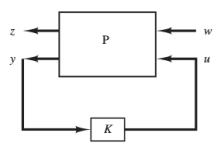
\includegraphics[scale=1.0]{generalizedPlant.jpg}
  \caption{Generalized plant dynamics}			
\end{figure}
\end{frame}
%
\begin{frame}{$H_{\infty}$ norm}
\begin{itemize}
\item $H_{\infty}$ norm is defined by: 
\end{itemize}
\begin{equation}
\|\Phi\|_{\infty} = \sup_{\omega}\bar{\sigma}[\Phi(jw)]
\end{equation}
\begin{figure}
  \center
  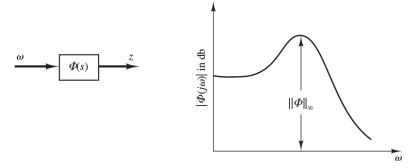
\includegraphics[scale=1.0]{HInf.jpg}
  \caption{Bode diagram and the $H_{\infty}$ norm}			
\end{figure}
\end{frame}
%
\begin{frame}{$H_{\infty}$ norm constraints}
\begin{itemize}
\item Assume multiplicative plant uncertainty $\Delta_m$ is bounded: $\bar{\sigma}[\Delta_m(jw)] < |W_m(jw)|$
\item Desire robust performance criterion: $\|S(jw)\|_{\infty} < W_s^{-1}$
\item We get
\end{itemize}
\begin{equation}
\left\| \begin{array}{c}
W_mT \\
W_sS \end{array} \right\|_{\infty} < 1
\end{equation}
\begin{itemize}
\item Similary $H_{\infty}$ constraint problems can be solved in multiple ways:
\begin{enumerate}
\item Riccati-type equations as in LQG (1980s)
\item Linear-Matrix Inequalities (LMI) (1990s)
\item Zero-sum differential game perspective yielding minmax controllers (most recent)
\end{enumerate}
\end{itemize}
\end{frame}
%
\section{Applications to Table Tennis?}
%
\begin{frame}{How to apply to table tennis?}
\begin{itemize}
\item Linear models of players may be inaccurate.
\item Robust control of switched linear systems!
\item Example: one for forehand and one for backhand dynamics.
\end{itemize}
\begin{figure}
  \center
  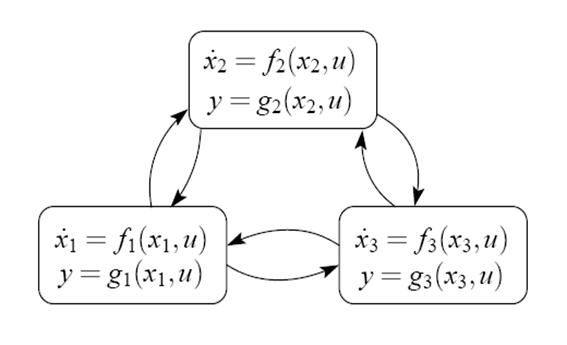
\includegraphics[scale=0.5]{hybridSystem.jpg}
  \caption{Switching dynamics}			
\end{figure}
\end{frame}
%
\begin{frame}{Conclusion}
\begin{itemize}
\item Thank you for listening!
\end{itemize}
\end{frame}	
%
\section{References}
\begin{frame}[allowframebreaks]{References}
\def\newblock{\hskip .11em plus .33em minus .07em}
\bibliographystyle{alpha}
\bibliography{myReferences} % file name of the bibtex
\end{frame}
%

%
% End of slides
\end{document} 